\documentclass{lecture_notes}

%==============================================================================%
% CONVENIENCE COMMANDS
%==============================================================================%
\newcommand{\vvec}{\vec{v}}
\newcommand{\rvec}{\vec{r}}
\newcommand{\omhat}{\hat{\Omega}}
\newcommand{\dom}{\dd \hat{\Omega}}
\newcommand{\de}{\dd E}
\newcommand{\dthree}{\dd^3}
\newcommand{\dtheta}{\dd \theta}
\newcommand{\dphi}{\dd \phi}
%==============================================================================%

\onehalfspacing

\title{NPRE 555: Reactor Theory I}
\subtitle{Lecture Notes}

\professor{Dr. Kathryn Huff}
\professortitle{Associate Professor in the Department of Nuclear, Plasma, \& Radiological Engineering}
\gradstudentcontribs{Liam Pohlmann}
\undergradstudentcontribs{}

\date{Fall 2025}

\begin{document}
\frontmatter

\begin{foreword}
  The purpose of this document is to contain the lecture notes given in NPRE 555: Reactor Theory I.
  It has been created by the students of this course on an ongoing basis throughout the semester.
  These notes are not intended to take the place of a true course on neutron transport.
  However, the hope is that this document will serve as a reference for those starting out or are otherwise familiar with the topic.
  These notes were created by Dr. Huff using her own experience and from references~\cite{bellNuclear_reactor_theory_bell_glasstone1970,duderstadtTransportTheory1979,lewisComputationalMethodsNeutron1993,staceyNuclearReactorPhysics2007}.
\end{foreword}

\tableofcontents
% \listoffigures
% \listoftables
\clearpage

% Start page numbering in arabic numerals
\pagestyle{fancy} % start main style
\fancyhf{}
\fancyfoot[C]{\thepage} % page numbers in footer
\pagenumbering{arabic}
\setcounter{page}{1}

\section{Definitions and Fundamentals}
The neutron population in any domain is governed by the linear Boltzmann transport equation, and the methods to solving this equation can be classified according to their discretization techniques, assumptions, etc.
\begin{figure}
  \centering
  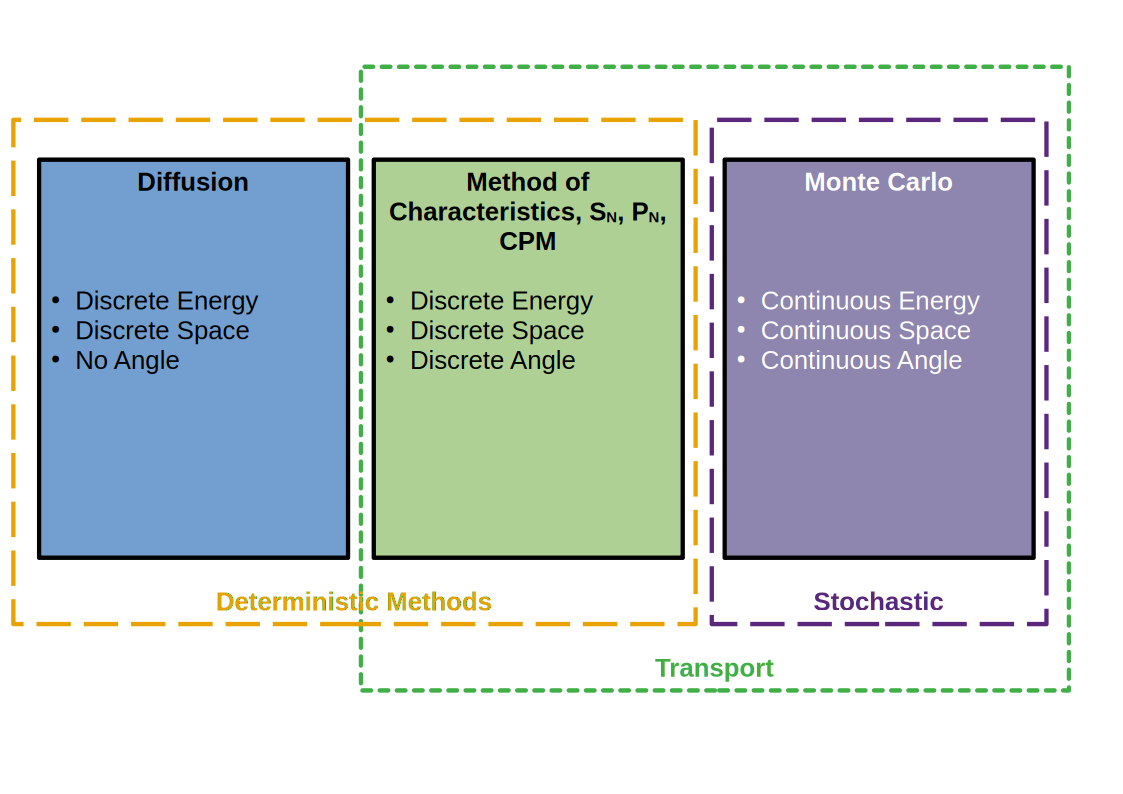
\includegraphics[width=\textwidth]{figs/transport_eq_methods_classification}
  \caption{Neutron population solver classifications}
  \label{fig:solver-classifications}
\end{figure}
To derive this equation, we first list the key assumptions\footnote{Note that these assumptions are only specific to this class. Applications outside of fission power reactors, such as particle colliders and fusion reactors, may see some of these simplifications break down.}:
\begin{enumerate}
  \item Particles are treated as \textit{points}. of this equation, we first list t
  \item Particles travel in straight lines between collisions.
  \item Particle-particle interactions are neglected.
  \item Collisions are instantaneous.
  \item Material properties are isotropic.
  \item Properties of nuclei and material compositions are time-independent.
  \item One the expectation (``mean'') value particle density will be considered
\end{enumerate}

\begin{definition}[Phase Space Density Function]\label{phase-space-density}
  $n(\rvec,\vvec,t)\dthree r \dthree v=$ the expected number of particles in $\dthree r$ about $r$ with velocity $\dthree v$ about v at time $t$.
\end{definition}
To simplify \cref{phase-space-density}, we then define the so-called ``solid angle'', $\omhat$:
\begin{equation} \label{eq:solid-angle}
  \omhat \equiv \frac{\vvec}{v}
\end{equation}
where $v=\norm{\vvec}$.
A visualization for this angle is given in \cref{fig:solid-angle}.
\begin{figure}
  \centering
  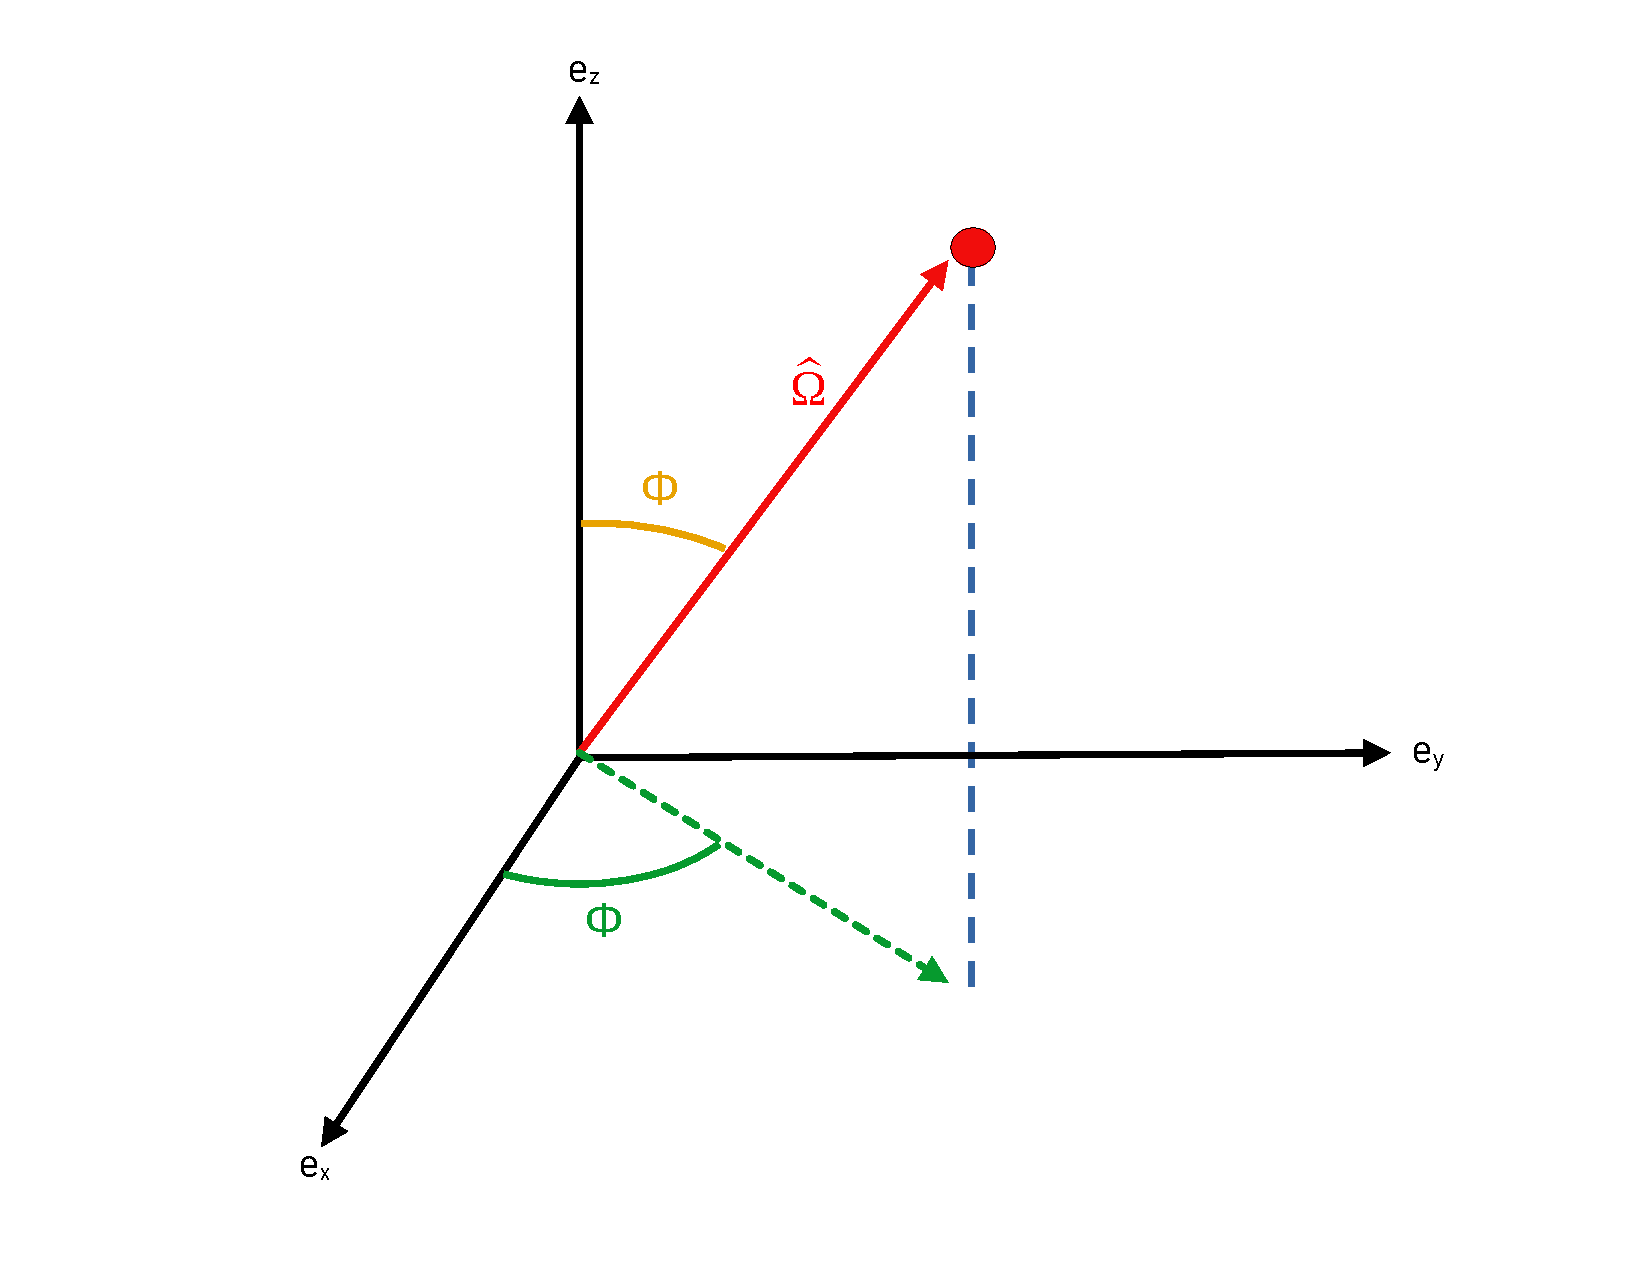
\includegraphics[width=\textwidth]{figs/solid_angle.pdf}
  \caption{Solid angle visualization.}
  \label{fig:solid-angle}
\end{figure}
The relation of the solid angle, which is given in spherical coordinates, to cartesian coordinates is:
\begin{equation}
  \omhat = \sin\theta \cos \phi \hat{e}_x+\sin\theta\sin\phi\hat{e}_y+\cos\theta\hat{e}_z
\end{equation}
while the differential element, $\dom$, is $\dom=\sin\theta \dtheta \dphi$.

With this and the energy, $E=\frac{1}{2}mv^2$, we then rewrite \cref{phase-space-density} as:
\begin{definition}[Phase Space Density Function -- Energy and Solid Angle]\label{phase-space-density-energy-solid-angle}
  $n(\rvec,\omhat,E,t)\dthree r \dom \de = $ the expected number of particles in $\dthree r$ about $r$ going in direction $\dom$ about $\omhat$ with energy $\de$ about $E$ at time $t$.
\end{definition}
Additional forms of \cref{phase-space-density,phase-space-density-energy-solid-angle} can be shown to be:
\begin{equation*}
  \begin{split}
    n(\rvec,E,\omhat,t) & = \frac{v}{m}n(\rvec,\vvec,t)         \\
    n(\rvec,E,\omhat,t) & = \frac{1}{mv}n(\rvec,\vvec,\omhat,t) \\
    n(\rvec,v,\omhat,t) & = v^2 n(\rvec,\vvec,t)
  \end{split}
\end{equation*}

\begin{definition}
  [Angular Current Density] \label{angular-current-density}
  The expected number of particles that cross an area $\dd S$ per second with velocity $\dthree v$ about $\vvec$ at time $t$.
  Symbol: $\vec{j}(\rvec,\vvec,t)\dd S, \dthree v$
\end{definition}
Rather than care about \textit{all} velocities, we might only care about the particular number of particles either coming in our out of our surface.
In which case, we define the \textit{partial current density}.
\begin{definition}
  [Partial Current Density]\label{partial-current-density}
  The rate at which particles flow through $S$ in the inward or outward direction.
  Symbol: $J_{\pm}(\rvec,t)$
\end{definition}
Using mathematical symbols, we can write \cref{angular-current-density} as:
\begin{equation}
  \label{eq:partial-current-density}
  J_{\pm}\equiv\pm \int_{\pm}\hat{e}_s\cdot \vec{j}(\rvec,\vvec,t)  \dthree v
\end{equation}
where $\hat{e}_s$ is the unit vector normal to the surface.
Note that because of the $\pm$ symbol in front of the integral, we are guaranteeing the quantity $\norm{J}$ to be positive.
\Cref{eq:partial-current-density} allows for further definition of \textit{net current density}:
\begin{equation}
  \label{eq:net-current-density}
  \vec{J}(\rvec,t)\cdot \hat{e}_s=J_+(\rvec,t)-J_-(\rvec,t)
\end{equation}

It is at this point we would like to urge extreme caution in the above definitions of neutron current, as the partial and net current densities are all \emph{scalar} quantities.
However, another common term is known as the \textit{neutron current density}, and is defined using the angular current density:
\begin{equation}
  \label{eq:neutron-current-density}
  \vec{J}(\rvec,E,t)\equiv \int_{4\pi}\vec{j}(\rvec,E,\omhat,t)\dom
\end{equation}
This new quantity is a \textbf{vector} describing the rate at which neutrons flow through a surface $\dd S$~\cite{duderstadtNuclearReactorAnalysis1976}.

A straightforward definition is the so-called \textit{angular flux}, which is simply the phase space density function scaled by the velocity:
\begin{equation}
  \label{eq:angular-flux}
  \psi\equiv vn(\rvec,\omhat,E,t)
\end{equation}
From this, we define the \textit{scalar flux}:
\begin{equation}
  \label{eq:scalar-flux}
  \Phi (\rvec,E,t)\equiv \int_{4\pi}\psi(\rvec,\omhat,E,t)\dom
\end{equation}

\section{The Boltzmann Transport Equation}
Consider a volume $V$ with surface $S$.
To determine the rate of change of $n(\rvec,\omhat,E,t)$, what phenomena must we consider?
\begin{enumerate}
  \item Collisions (ex. absorption, elastic/inelastic scatter)
  \item Streaming (moving in and out of the volume through the surface)
  \item Sources
\end{enumerate}

\clearpage
\appendix

\clearpage
\bibliographystyle{ieeetr}
\bibliography{NPRE_555}
\end{document}
